\documentclass{standalone}
\usepackage{pgfplots}
\pgfplotsset{compat=1.13}
\usepackage{amsmath}

\begin{document}

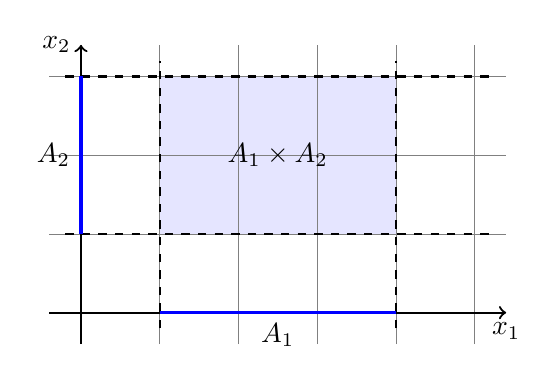
\begin{tikzpicture}
    \fill[blue!10!white] (1,1) rectangle (4,3);
    \draw[step=1cm,gray,very thin] (-0.4,-0.4) grid (5.4,3.4);
    \draw[thick,->] (-0.4,0) -- (5.4,0) node[anchor=north]{\(x_1\)};
    \draw[thick,->] (0,-0.4) -- (0,3.4) node[anchor=east]{\(x_2\)};
    \draw[thick,dashed] (1,-0.2) -- (1,3.2);
    \draw[thick,dashed] (4,-0.2) -- (4,3.2);
    \draw[thick,dashed] (-0.2,1) -- (5.2,1);
    \draw[thick,dashed] (-0.2,3) -- (5.2,3);
    \draw[blue, very thick] (1,0) -- (4,0) node[black,midway,below]{\(A_1\)};
    \draw[blue, very thick] (0,1) -- (0,3) node[black,midway,left]{\(A_2\)};
    \node[] at (2.5,2) {\(A_1 \times A_2\)};
\end{tikzpicture}

\end{document}